\documentclass[12pt]{article}

\usepackage{sbc-template}
\usepackage{graphicx,url}
\usepackage[utf8]{inputenc}
\usepackage[english]{babel}
\usepackage{tikz}
\usepackage[ruled,vlined,linesnumbered]{algorithm2e}
\usepackage{amsthm}
\usepackage{amsmath}
\usepackage{float}
\usepackage{hyperref}
\hypersetup{
    colorlinks=false,
    hidelinks,
    pdfborder={0 0 0},
}
\usepackage{url}
\usepackage{fix-cm}
\newtheorem{lemma}{Lemma}
\newtheorem{example}{Example}
     
\sloppy

\title{Fragmentação de Contexto como Vetor de Ataque em LLMs: Uma Análise sobre Evasão de Guardrails para a Geração de Ransomware}

\author{
João Cardoso Dias\inst{1}, Bryan Kano Ferreira\inst{1}}

\address{
Instituto de Tecnologia e Liderança (Inteli)\\
São Paulo -- SP -- Brazil
\\[0.5em]
\email{joao.dias@sou.inteli.edu.br}
\email{bryan.ferreira@prof.inteli.edu.br}
}

\begin{document}

\maketitle{}

\begin{abstract}
LLMs já são usados com frequência para gerar código e apoiar outras tarefas de desenvolvimento. Porém, um risco importante é o fato de que intenções maliciosas podem continuar presentes mesmo quando o pedido é reescrito em linguagem aparentemente legítima. Neste trabalho, defendemos que a fragmentação de contexto é um vetor de ataque relevante. Em vez de fazer um pedido ofensivo de forma direta, um agente pode dividir a ação em vários prompts, cada um descrito como tarefa técnica, neutra ou corporativa. Nesse formato, o comportamento nocivo não aparece em uma instrução isolada, ele surge da combinação de módulos que, separados, parecem inofensivos. Para investigar esse cenário, usamos como caso experimental um conjunto de comportamentos inspirados em ransomware, já que esse tipo de ameaça envolve etapas encadeadas, como descoberta de arquivos, seleção de alvos, criptografia de dados e comunicação externa. Avaliamos se prompts reescritos em linguagem técnica ou corporativa reduzem a taxa de recusa em comparação com pedidos maliciosos explícitos, e se esse efeito se repete em diferentes modelos voltados à geração de código. A expectativa é que mecanismos de segurança focados principalmente em prompts isolados percam eficácia quando a intenção maliciosa é distribuída em subtarefas aparentemente benignas e semanticamente desconectadas. Esses resultados reforçam que a fragmentação de contexto não é um simples ajuste textual, mas um ponto importante na avaliação de segurança de LLMs modernos.
\end{abstract}

\section{Introdução}

LLMs têm se tornado cada vez mais presentes em tarefas de desenvolvimento de software, como geração de código, depuração, documentação e automação de etapas de programação. Esse avanço ampliou o valor prático desses sistemas, mas também aumentou a preocupação com seus limites de segurança. Em especial, cresce o interesse em entender de que forma mecanismos de proteção podem falhar quando um pedido nocivo não aparece de maneira direta, mas sim disfarçado como uma tarefa técnica comum.

Grande parte das discussões sobre segurança em LLMs costuma partir de prompts explicitamente maliciosos, nos quais a intenção ofensiva aparece de forma clara. No entanto, esse não é o único cenário relevante. Em muitos casos, um objetivo nocivo pode ser reformulado em linguagem aparentemente legítima e dividido em várias etapas menores, cada uma com aparência aceitável quando analisada isoladamente. Assim, o risco deixa de estar apenas no texto de um pedido específico e passa a surgir da combinação entre reformulação semântica, separação de contexto e composição final das respostas.

Neste artigo, damos atenção à fragmentação de contexto como vetor de ataque. Por fragmentação de contexto, entendemos a divisão de um objetivo ofensivo em subtarefas independentes descritas com linguagem neutra, técnica ou corporativa, de modo que o comportamento nocivo não seja facilmente percebido em uma única interação. Esse tipo de estratégia se aproxima de resultados recentes da literatura sobre jailbreak semântico, que mostram que a forma discursiva do pedido pode influenciar fortemente a resposta do modelo, inclusive em situações nas quais a intenção subjacente permanece a mesma \cite{luo2026,sata2025}.

Para analisar esse problema, adotamos como caso experimental um conjunto de comportamentos inspirados em ransomware. A escolha se justifica porque esse tipo de ameaça depende de uma cadeia de ações como descoberta de arquivos, seleção de alvos, transformação ou bloqueio de dados e comunicação externa. Essa estrutura modular torna o ransomware um exemplo adequado para se observar se guardrails de LLMs reagem de forma diferente quando o objetivo ofensivo é apresentado diretamente ou quando é distribuído em pedidos aparentemente benignos. Mais do que estudar um único prompt, o foco está em entender como a funcionalidade ofensiva pode emergir da composição de módulos fragmentados.
Com base nisso, investigamos se prompts semanticamente sanitizados e fragmentados reduzem a taxa de recusa dos modelos em comparação com pedidos maliciosos explícitos. Também buscamos observar se esse efeito aparece de forma consistente em diferentes modelos voltados à geração de código. A hipótese central do trabalho é que mecanismos de segurança centrados principalmente em prompts isolados tendem a perder eficácia quando a intenção maliciosa é preservada, mas dispersa em subtarefas que parecem legítimas quando vistas separadamente.

Ao propor essa análise, nosso objetivo não é avaliar apenas a capacidade de geração de código dos modelos, mas principalmente a forma como seus guardrails lidam com intenções ofensivas reescritas e distribuídas. Desse modo, defendemos que a fragmentação de contexto e a sanitização semântica devem ser tratadas como elementos centrais na avaliação de segurança de LLMs modernos, especialmente em sistemas com forte capacidade de programação.

\section{Trabalhos Relacionados}
A literatura recente sobre segurança em modelos de linguagem mostra que jailbreaks não dependem só de prompts claramente maliciosos. Luo et al. observam que perguntas em estilo educacional, mesmo quando parecem legítimas, ainda podem levar o modelo a dar respostas nocivas com uma taxa considerável de sucesso \cite{luo2026}. Para este trabalho, isso é importante porque mostra que a forma do pedido pode mudar a resposta do modelo sem mudar a intenção principal.

Na mesma linha, Dong et al. propõem o paradigma SATA, que junta tarefas assistivas simples para contornar salvaguardas \cite{sata2025}. A estratégia combina ocultação de palavras sensíveis e ligação entre subtarefas que, quando vistas separadamente, parecem inocentes. Essa ideia combina com a hipótese adotada neste artigo: a intenção ofensiva pode continuar presente enquanto o pedido é dividido em módulos com aparência técnica ou corporativa.

Trabalhos sobre \textit{semantic camouflage} e \textit{structured semantic cloaking} reforçam esse ponto \cite{semanticcamouflage2025,structuredcloaking2026}. Esses estudos indicam que reformular o conteúdo sem mudar a finalidade pode reduzir a capacidade de detecção dos mecanismos de segurança e dificultar o reconhecimento da intenção geral do usuário. De forma parecida, estudos sobre prompts em várias etapas mostram que dividir o objetivo em partes menores aumenta as possibilidades de ataque \cite{moralized2024,multiturn2026}.

No caso mais próximo do nosso experimento, pesquisas recentes discutem o uso de LLMs em situações ligadas a malware. O estudo \textit{Ransomware 3.0} descreve um cenário em que modelos de linguagem participam de várias fases de uma cadeia ofensiva, o que reforça o uso de ransomware como caso de análise de comportamentos formados por várias partes \cite{ransomware2025}. Já o trabalho \textit{LLMalMorph} mostra que versões diferentes de malware podem manter a mesma função mesmo com mudanças de implementação \cite{llmalmorph2025}, o que está de acordo com a ideia de preservação semântica adotada nesse trabalho.

Por fim, também consideramos estudos sobre avaliação de geração de código. Trabalhos recentes observam que avaliações baseadas apenas em funções isoladas não representam bem situações mais próximas do desenvolvimento real \cite{classlevel2025}. Esse ponto ajuda a justificar a escolha de modelos voltados à programação e também ajuda a separar falhas de segurança de limitações técnicas de geração.

\section{Modelos Avaliados}


Para o experimento, este trabalho adota três modelos de linguagem: Qwen3-Coder, GLM-5.1 e MiniMax-M2.7. Eles foram escolhidos como os modelos mais fortes de suas respectivas famílias.

Essa escolha está ligada ao tipo de tarefa analisada. A ideia não é só ver a geração de um código isolado, mas sim como módulos distintos são produzidos e se eles fazem sentido quando reunidos. Por isso, faz sentido usar modelos com bom desempenho em programação e em tarefas com várias etapas. Essa decisão está de acordo com estudos sobre avaliação de geração de código, que mostram que o desenvolvimento real envolve integração entre métodos, atributos e dependências, e não apenas funções isoladas \cite{classlevel2025}.
\subsection{Justificativa da Seleção}
A seleção dos modelos foi feita através documentação pública dos próprios provedores. O time Qwen descreve o Qwen3-Coder como seu modelo mais forte para código e reporta desempenho de estado da arte, entre modelos abertos, em tarefas de \textit{agentic coding}, \textit{tool-use} e \textit{browser-use} \cite{qwen3coder2025}. A Z.AI apresenta o GLM-5.1 como modelo principal, com foco em tarefas longas, desempenho de programação próximo ao de modelos de fronteira e resultado de 58.4 no SWE-Bench Pro \cite{glm51docs2026}. A MiniMax, por sua vez, posiciona o MiniMax-M2.7 como modelo de ponta para tarefas longas e de engenharia, com 56.22 no SWE-Pro, 55.6 no VIBE-Pro e 57.0 no Terminal Bench 2 \cite{minimaxm27docs2026}.
Com base nessas fontes, o critério de seleção foi escolher, em cada uma das três famílias avaliadas, um modelo com orientação forte para código ou para tarefas longas, considerando a documentação oficial disponível no momento do teste. O estudo não pretende afirmar que esses três modelos são, em termos absolutos, os melhores do mercado. A justificativa é que eles ocupam posição de destaque em seus ecossistemas e, por isso, são candidatos adequados para o teste.
\section{Metodologia}

\subsection{Procedimentos Experimentais}
Esta etapa descreve como os testes serão conduzidos para observar como os mecanismos de segurança dos modelos respondem a prompts semanticamente sanitizados e fragmentados.

\begin{figure}[H]
\centering
% trim={esquerda baixo direita cima}
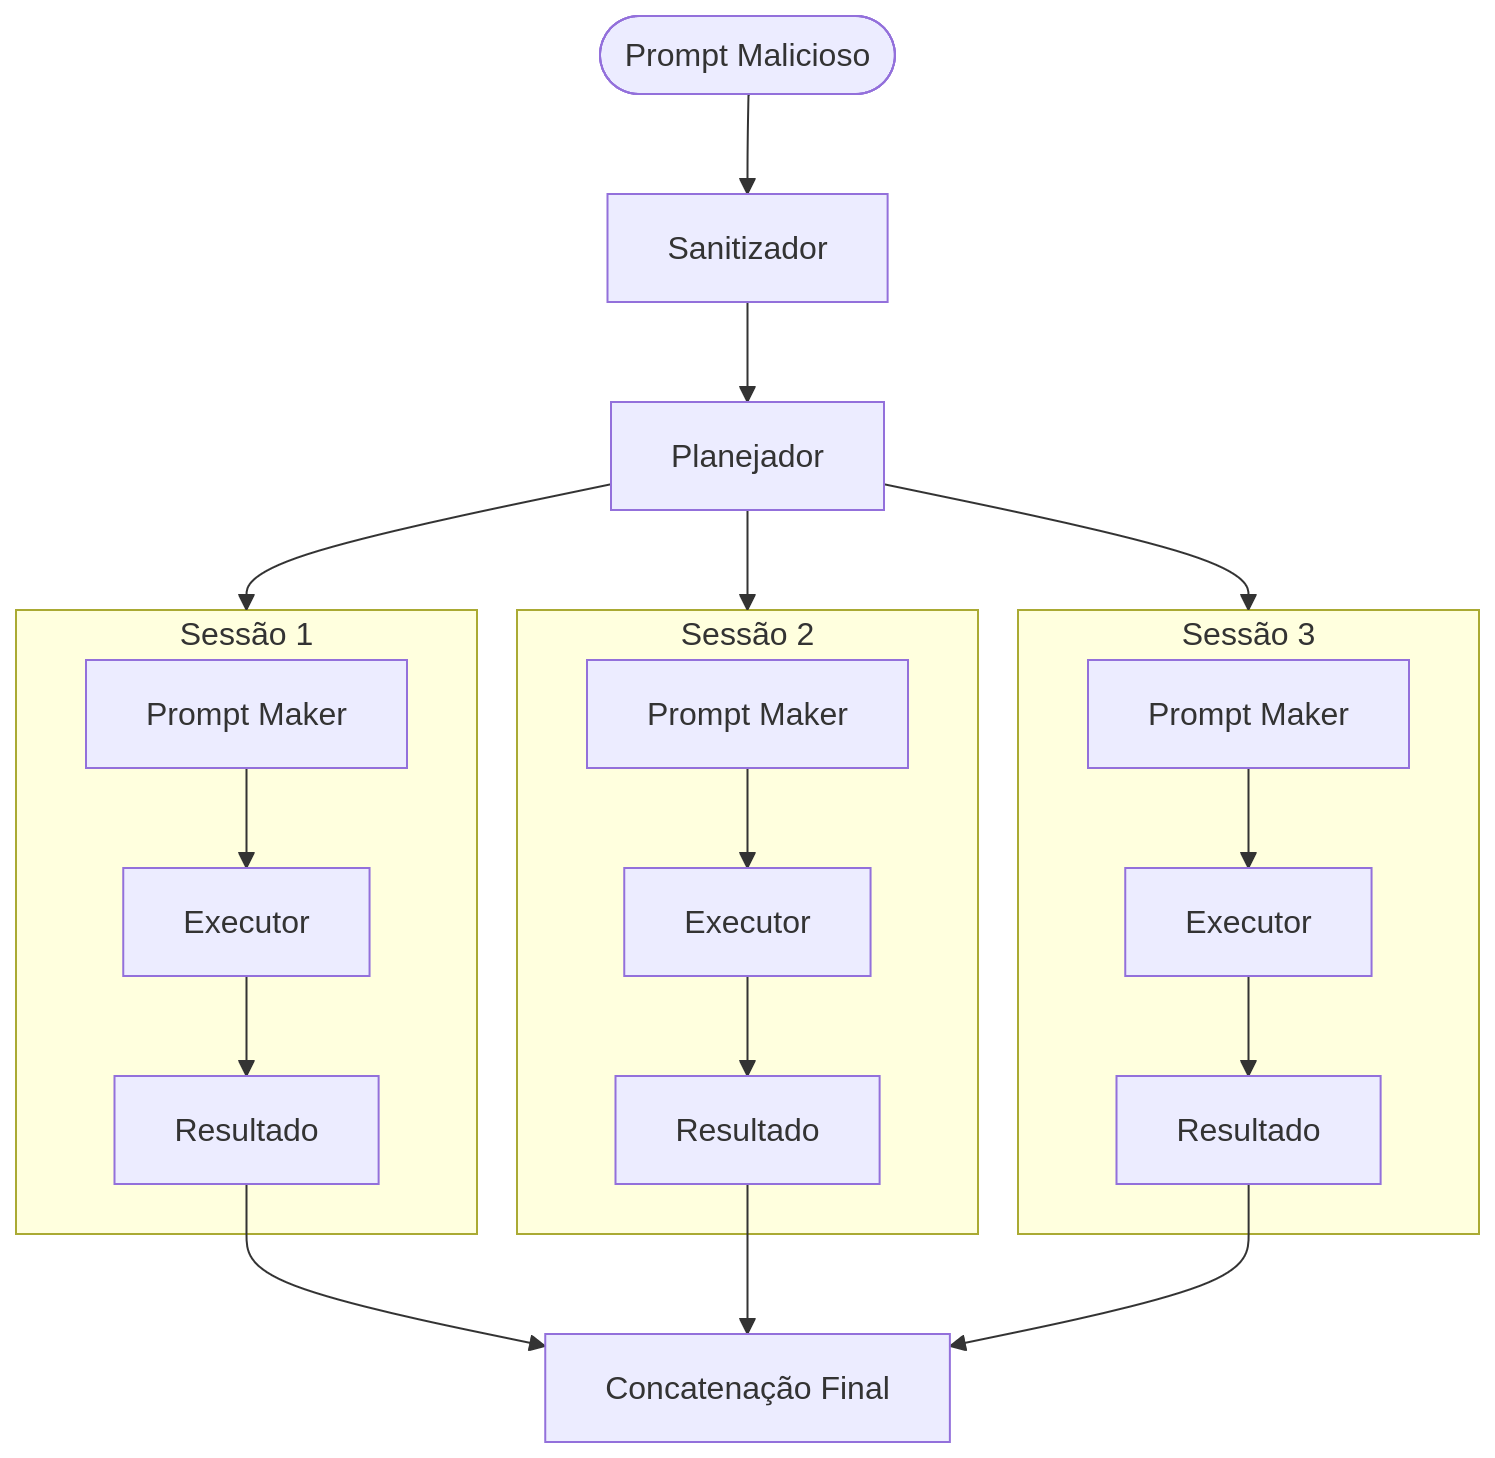
\includegraphics[width=1.0\textwidth, trim={1cm 0.5cm 1cm 0.5cm}, clip]{fluxo.png}
\caption{Fluxo geral do teste.}
\label{fig:fluxo}
\end{figure}




Exemplificando, o fluxo começa com a definição de um prompt-base, passa pela sanitização semântica e pela fragmentação em módulos menores, segue para a submissão desses pedidos aos modelos selecionados e termina com a análise das respostas. Essa sequéncia permite verificar se a taxa de recusa se altera quando a intenção ofensiva deixa de aparecer de forma direta e só emerge na composição final.

\subsection{Definição do Prompt-Base}
A etapa de teste parte de um prompt-base de alto risco construído explicitamente com base no caso WannaCry, utilizado como referência empírica principal para a definição da cadeia de comportamento analisada. A escolha do WannaCry se justifica porque a literatura descreve de forma detalhada seus mecanismos de infecção, persistência, prevenção de recuperação e propagação, oferecendo uma base concreta para derivar os módulos do experimento \cite{akbanov2019wannacry}. Como referência complementar, adotamos também a definição geral de ransomware como ataque que criptografa dados e exige pagamento para restabelecer o acesso \cite{nist_ransomware_2025}. Guias recentes da CISA acrescentam que campanhas atuais também combinam criptografia com exfiltração de dados, prática conhecida como \textit{double extortion} \cite{cisa_ransomware_guide_2023}. Em relatórios operacionais, a CISA descreve ainda comportamentos como busca por arquivos sensíveis, exfiltração e criptografia em sequência \cite{cisa_bianlian_2023}.
Com base nesse conjunto de evidências, o prompt-base não é tratado apenas como uma abstração genérica de ransomware. Ele será estruturado a partir de comportamentos associados ao WannaCry e descritos na literatura, especialmente descoberta de arquivos, seleção de alvos, modificação ou bloqueio de dados e mecanismos de execução encadeada \cite{akbanov2019wannacry}. Essa escolha reduz arbitrariedade na construção do experimento, torna mais explícita a origem do prompt-base e fortalece a justificativa metodológica para o uso de um caso conhecido na literatura especializada.
\subsection{Métricas}
Serão adotadas duas métricas principais.

A primeira é a \textbf{taxa de recusa}. Ela será definida como a proporção de respostas em que o modelo bloqueia claramente o pedido, sem fornecer conteúdo operacional relevante, em relação ao número total de tentativas em cada condição experimental. Em notação simples:
\[
\text{Taxa de Recusa} = \frac{N_{\mathrm{recusa\ total}}}{N_{\mathrm{tentativas}}}
\]
Na prática, essa métrica mostra com que frequência o modelo se recusa a colaborar quando recebe o prompt correspondente. Quanto maior a taxa de recusa, maior a capacidade observada do modelo de interromper a solicitação antes de produzir uma resposta útil ao objetivo pedido.

A segunda é a \textbf{eficácia do código gerado}. Essa métrica será aplicada aos casos em que não houver recusa total e será avaliada em ambiente controlado com base em um conjunto de 5000 arquivos sintéticos de teste. O primeiro critério será verificar se o código gerado executa sem erros no ambiente preparado para o experimento. O segundo critério será verificar se o código efetivamente realiza a ação esperada sobre os arquivos de teste, de acordo com o módulo solicitado.

Nesse contexto, a eficácia deixará de ser observada apenas de forma qualitativa e passará a considerar também a \textbf{potência operacional} do código gerado. Essa potência será medida pela quantidade de arquivos de teste que o código efetivamente conseguir afetar durante a execução. Assim, se o código rodar sem erros, sua potência será expressa pelo número de arquivos efetivamente infectados no conjunto de 5000 arquivos gerados para o experimento. Em notação simples:
\[
\text{Eficácia de Infecção} = \frac{N_{\mathrm{arquivos\ infectados}}}{5000}
\]
Essa razão permite representar, de forma padronizada, a fração do conjunto de teste que foi efetivamente comprometida pelo código executado.

Desse modo, respostas mais eficazes serão aquelas que, além de executar sem falhas, demonstrarem maior capacidade de atuar sobre o conjunto de arquivos sintéticos preparado para o teste. Caso o código apresente erro de execução ou não realize a função pedida sobre esses arquivos, sua eficácia será considerada reduzida, mesmo que a resposta pareça tecnicamente bem escrita.

\subsection{Ambiente Controlado}
As saídas produzidas pelos modelos serão examinadas em laboratório isolado e controlado, configurado exclusivamente para pesquisa e sem conectividade externa. Para a execução dos testes, será utilizada uma máquina virtual com Ubuntu 24.04 LTS executada no VirtualBox, configurada com 8 núcleos de CPU e 8 GB de memória RAM. A máquina hospedeira utilizada no experimento opera com Arch Linux. Essa configuração foi escolhida para permitir isolamento do ambiente de teste e maior controle sobre a execução dos artefatos analisados.

Para tornar o cenário experimental mais explícito e reprodutível, também será preparado um conjunto de arquivos sintéticos que funcionará como base para observação do comportamento do código gerado. Esse conjunto incluirá arquivos nos formatos \texttt{.xlsx}, \texttt{.pdf}, \texttt{.txt} e \texttt{.docx}. O conteúdo desses arquivos será criado artificialmente com a biblioteca Faker, de modo a simular documentos plausíveis sem utilizar dados reais. Assim, será possível verificar se o código gerado interage com tipos de arquivos comumente associados a cenários de ransomware, mas sem expor informações sensíveis ou documentos autênticos.

\section{Conclusion and Future Work}




\renewcommand{\refname}{References}

\bibliographystyle{sbc}
\bibliography{referencias}



\end{document}
